\subsection{Khảo sát công nghệ xây dựng cốt lõi}

\subsubsection{Mô hình ngôn ngữ lớn (Large Language Model)}

Năm 2017, các kỹ sư của
\textbf{
\textcolor{blue}{G}%
\textcolor{red}{o}%
\textcolor{yellow}{o}%
\textcolor{blue}{g}%
\textcolor{green}{l}%
\textcolor{red}{e}
}
đưa ra bài báo \enquote{Attention Is All You Need}
khai sinh kiến trúc Transformer
với cơ chế tự chú ý Self-Attention,
mở đường cho hầu hết kiến trúc
LLM (Large Language Model) hiện nay.
Cách hoạt động của LLM
là dự đoán xác suất của từ tiếp theo
dựa theo các từ đã xuất hiện trước đó.
LLM không đọc chữ như con người.
Chia câu thành các phần nhỏ gọi là token.
Biến mỗi token thành vector
trong không gian nhiều chiều.
Những từ có nghĩa gần nhau
vua (king) và hoàng hậu (queen), hoặc mèo (cat) và chó (dog)
sẽ có các tọa độ rất gần nhau trong không gian.

\begin{figure}[H]
\centering
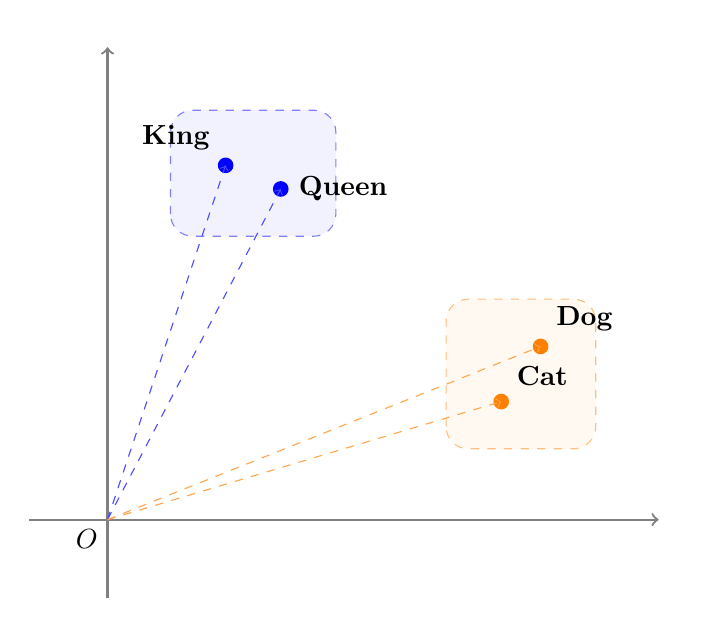
\begin{tikzpicture}[
scale=1, % Phóng to toàn bộ tọa độ lên 1 lần
every node/.style={scale=1}, % Phóng to chữ và node theo tỷ lệ tương ứng
% >=Stealth,
dot/.style={circle, fill=#1, inner sep=2pt},
cluster/.style={dashed, draw=#1!50, fill=#1!5, rounded corners=8pt, inner sep=6pt}
]

% --- Hệ Trục Tọa Độ ---
\draw[->, thick, gray] (-1,0) -- (7,0) node[right, black] {};
\draw[->, thick, gray] (0,-1) -- (0,6) node[above, black] {};
\node[below left] at (0,0) {$O$};

\coordinate (king) at (1.5, 4.5);
\coordinate (queen) at (2.2, 4.2);

\draw[cluster=blue] (0.8, 3.6) rectangle (2.9, 5.2);
\node[blue!80!black, above] at (1.85, 5.2) {};

% Vẽ các điểm và nhãn
\node[dot=blue, label={above left:\textbf{King}}] at (king) {};
\node[dot=blue, label={right:\textbf{Queen}}] at (queen) {};

% Vẽ vector từ gốc tọa độ (tùy chọn để thể hiện tính chất vector)
\draw[->, blue!70, dashed] (0,0) -- (king);
\draw[->, blue!70, dashed] (0,0) -- (queen);

% --- Cụm 2: Thú cưng (Cat và Dog) ---
% Định nghĩa tọa độ cho Cat và Dog nằm rất gần nhau nhưng xa cụm King/Queen
\coordinate (cat) at (5.0, 1.5);
\coordinate (dog) at (5.5, 2.2);

% Vùng không gian chung cho cụm Thú cưng
\draw[cluster=orange] (4.3, 0.9) rectangle (6.2, 2.8);
\node[orange!80!black, above] at (5.25, 2.8) {};

% Vẽ các điểm và nhãn
\node[dot=orange, label={above right:\textbf{Cat}}] at (cat) {};
\node[dot=orange, label={above right:\textbf{Dog}}] at (dog) {};

% Vẽ vector từ gốc tọa độ
\draw[->, orange!70, dashed] (0,0) -- (cat);
\draw[->, orange!70, dashed] (0,0) -- (dog);

% % --- Chú thích khoảng cách ---
% % Vẽ mũi tên hai đầu thể hiện khoảng cách gần nhau trong cụm
% \draw[<->, red, thick] (king) -- node[above right, scale=0.7] { } (queen);
% \draw[<->, red, thick] (cat) -- node[above left, scale=0.7] { } (dog);

\end{tikzpicture}

\caption{Ví dụ ánh xạ các vector từ gần nghĩa.}
\end{figure}

Trong đồ án này, em dùng
mô hình
HuggingFace (keepitreal/vietnamese-sbert)
tạo vector nhúng (embedding) cho tiếng Việt
với
số chiều (dimension) của mỗi vector là 768.

Khi dự đoán từ tiếp theo,
mô hình không chỉ nhìn vào từ ngay trước nó,
mà nó nhìn vào toàn bộ các từ đã xuất hiện và dùng cơ chế gọi là Self-Attention để xem từ nào quan trọng nhất.
Ví dụ: Trong câu \enquote{Con mèo rượt đuổi con chuột vì nó chạy rất nhanh}, cơ chế Attention sẽ giúp mô hình hiểu chữ \enquote{nó} ở đây có xác suất cao là đang chỉ \enquote{con chuột} chứ không phải \enquote{con mèo}.
Sau khi tính toán ngữ cảnh, mô hình sẽ quét qua toàn bộ kho từ vựng và gán cho mỗi từ một con số xác suất. Mô hình sẽ chọn từ tiếp theo dựa trên bảng xác suất này. Quá trình này lặp đi lặp lại liên tục cho đến khi nó tạo ra một ký tự đặc biệt ra lệnh dừng lại.

\begin{figure}[H]
\centering
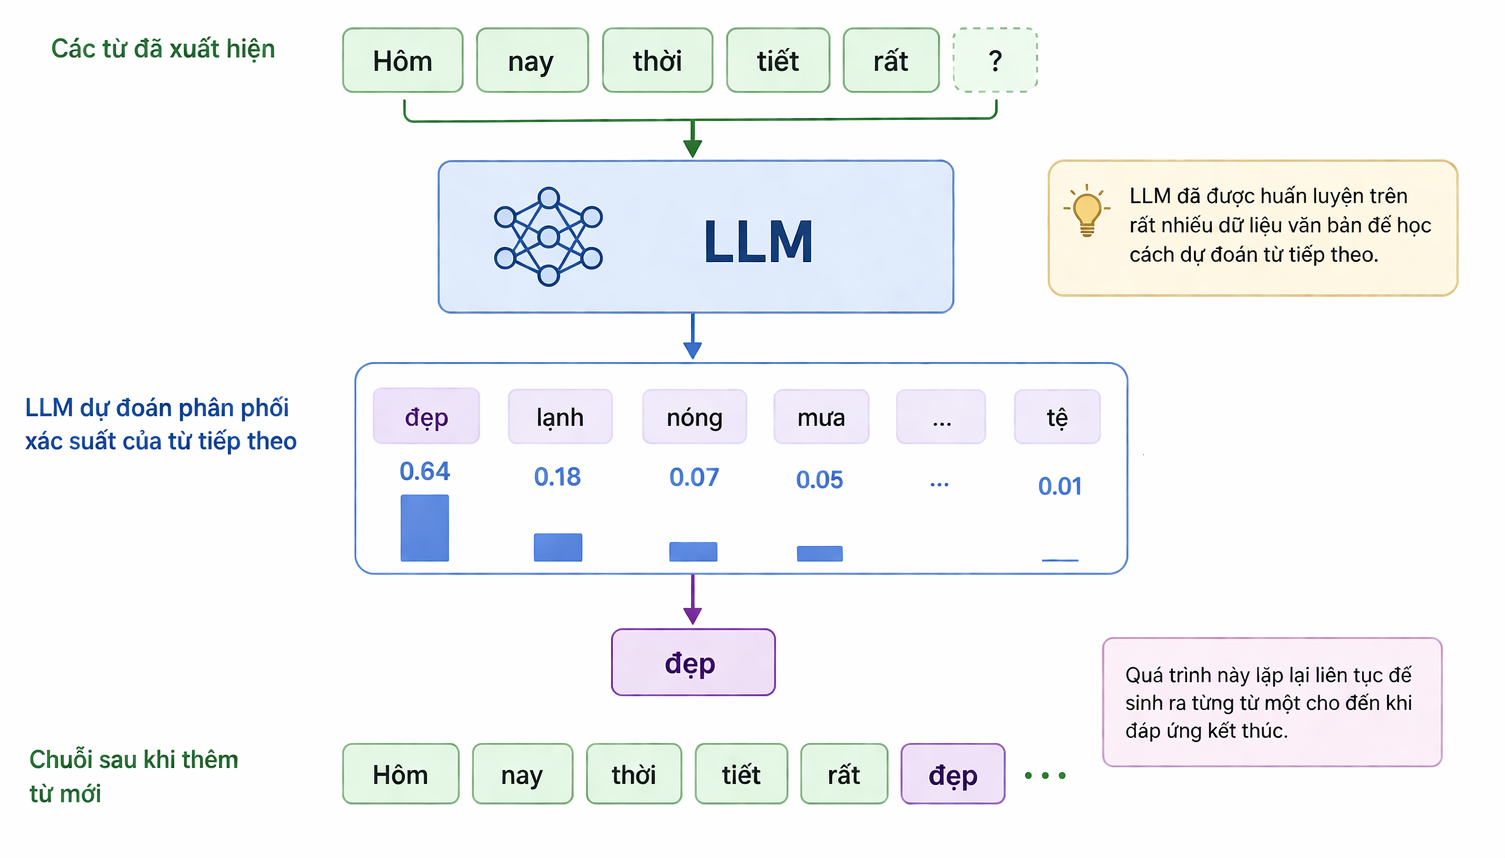
\includegraphics[scale = 0.4]{pictures/llm.png}
\caption{Cách hoạt động của LLM}
\end{figure}

Tuy nhiên LLM có một số nhược điểm:

\begin{itemize}

\item Dữ liệu huấn luyện rộng

\item Độ chính xác không cao với miền cụ thể

\item Có hiện tượng ảo giác (Hallucination)

\item Dữ liệu chỉ cập nhật đến ngày train (dữ liệu cũ)

\item LLM không biết dữ liệu mới

\item LLM không biết dữ liệu doanh nghiệp

\item LLM không biết tài liệu người dùng

\item Chi phí cho việc huấn luyện, tinh chỉnh lớn.

\end{itemize}

\begin{figure}[H]
\centering
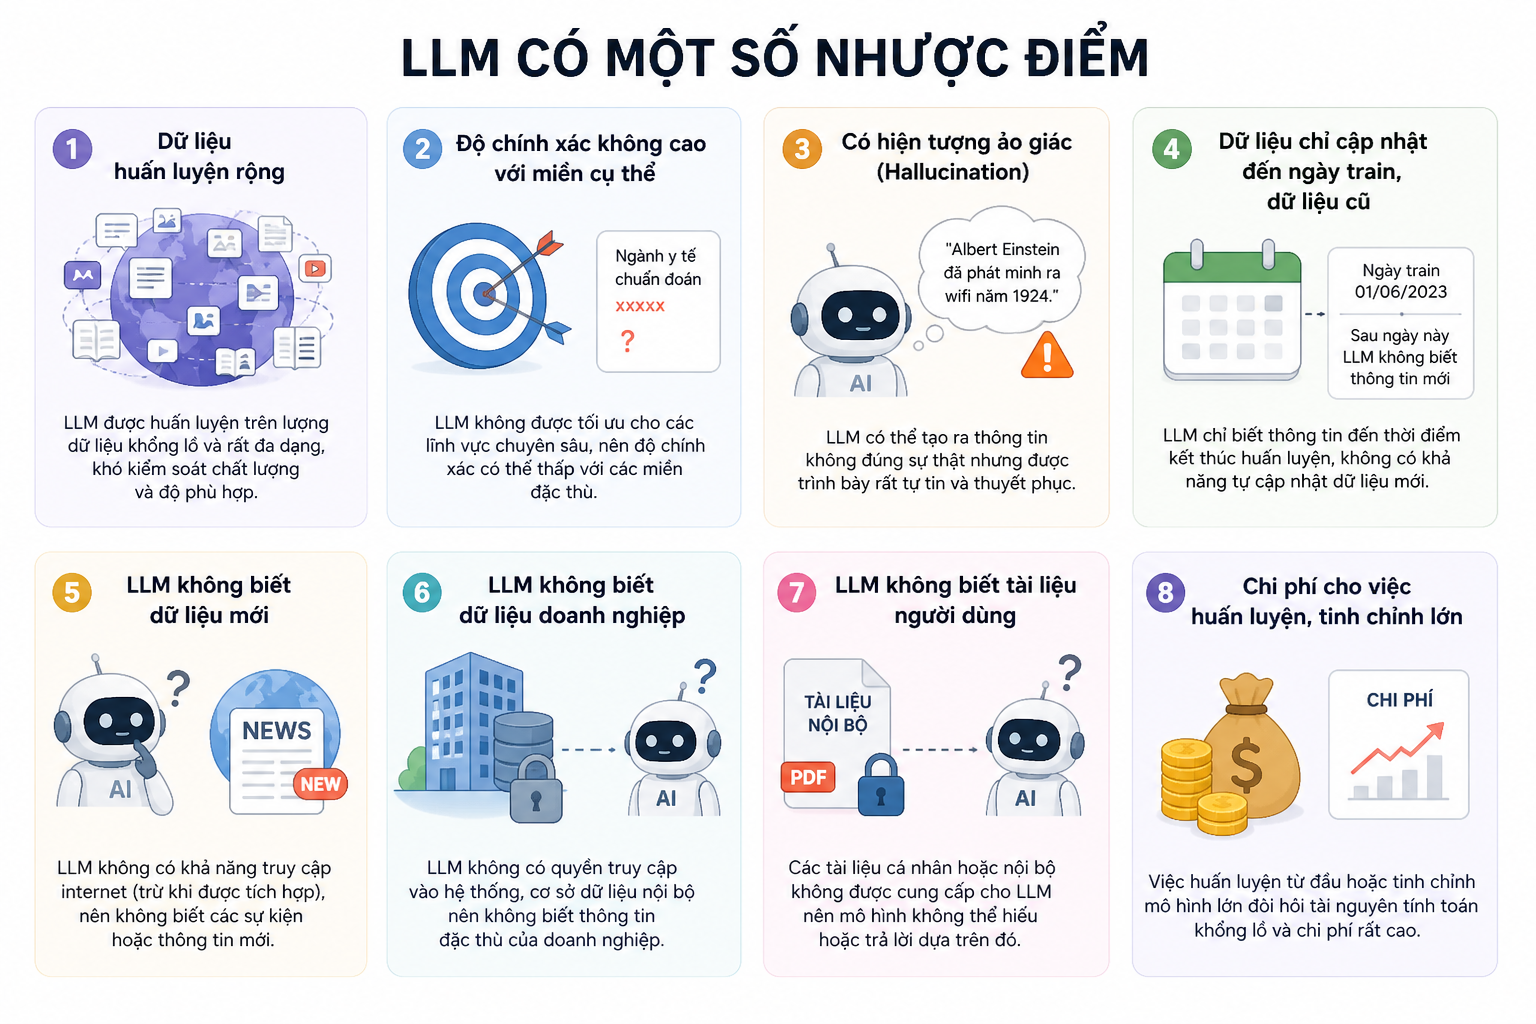
\includegraphics[scale = 0.25]{pictures/llm-crons.png}
\caption{Một số nhược điểm của LLM}
\end{figure}
